\documentclass[10pt,conference,compsocconf]{IEEEtran}

\usepackage{hyperref}
\usepackage{graphicx}
\usepackage{amsmath}
\usepackage{amsfonts}
\usepackage{amssymb}
\usepackage{subfig}
\usepackage{cite}
\begin{document}
\title{Spatially-Inferred Graphical Models for fMRI Data Mining}

\author{
  Pedro Abranches de Carvalho, Hongyu Luo and Roser Vi\~nals Terr\'es\\
  \textit{\'Ecole polytechnique f\'ed\'erale de Lausanne, Switzerland}

}

\maketitle

\begin{abstract}

Functional Magnetic Resonance Imaging (fMRI) offers the possibility to record neural activity in the human brain. This activity occurs in the shape of spatially organized patterns; networks of brain regions interact dynamically. In particular, some regions cause others to activate or de-activate. In this project, we consider the problem of inferring this causality using graphical Granger modeling. In other words, we want to unravel whether an fMRI signal from a given region can be predicted using signals from other regions. This boils down to the problem of learning causality matrices from a collection of spatio-temporal time-series. We tackle this task by minimizing a functional incorporating a data-fidelity term that fits the signals to a vector-auoregressive (VAR)  model and an $\ell_1$-regularization term. Such regularity prior forces the causality matrix to have sparse entries. This is in line with the fact that a given region in the brain is expected to have causal influences from very few other regions. We tested the algorithm on simplistic synthetic data to assess the performance, before applying to real Resting-State fMRI data from healthy subjects. The estimated causality matrix was then used to study causal effects between known large-scale activation networks. The results uncover insightful network-to-network causal couplings. 


\end{abstract}

\section{Introduction}
Human brain is a complex system. Intrinsic and spontaneous brain activation can be recorded using functional magnetic resonance imaging (fMRI) through the fluctuations of blood-oxygen-level dependent (BOLD) signals. 

Modeling the resting-state fMRI is crucial to understand the regional interactions of temporal brain activation. In this project, we use network modeling and dynamical analysis to infer the temporal-spatial causality from time series activation on different brain regions based on resting state fMRI. 

With the purpose of inferring causality between brain regions, we use graphical Granger causality (GC) modeling. GC is based on the fact that when, considering the past temporal samples of a signal improves the predictability of the future time samples of another signal, the first is causing the second. Mathematically, this approach can be formulated using vector autoregressive (VAR) modeling, that accounts multiple linear dependencies between multiple time series. 

Granger Causality has been widely used for fMRI ~\cite{deshpande2010effect, roebroeck2005mapping, hamilton2011investigating,wen2013granger,deshpande2009multivariate}. However, in this project we introduce a novel application of GC for the estimation of brain causality. Our work differs with the existing literature mainly in two aspects. First, we use deconvolved signals which reflect the activity moments, undone from the effect of haemodynamics \cite{karahanouglu2013total}. Second, we study causality between innovation-driven co-activation patterns (iCAPs), patterns that reveal spatially and temporally overlapping large-scale networks \cite{icap}. Figure \ref{fig:task_graph} shows the main pipeline of this project.

The rest of the paper is organized as follows. Section \ref{sec:Spatio-temporal} describes the spatio-temporal modeled and formulates the problem. Section \ref{sec:data} describes the fMRI data used and the synthetic data generated for verifying our approach. Section \ref{sec:results} presents the results and Section \ref{sec:summary} concludes the paper.


\begin{figure}
    \centering
    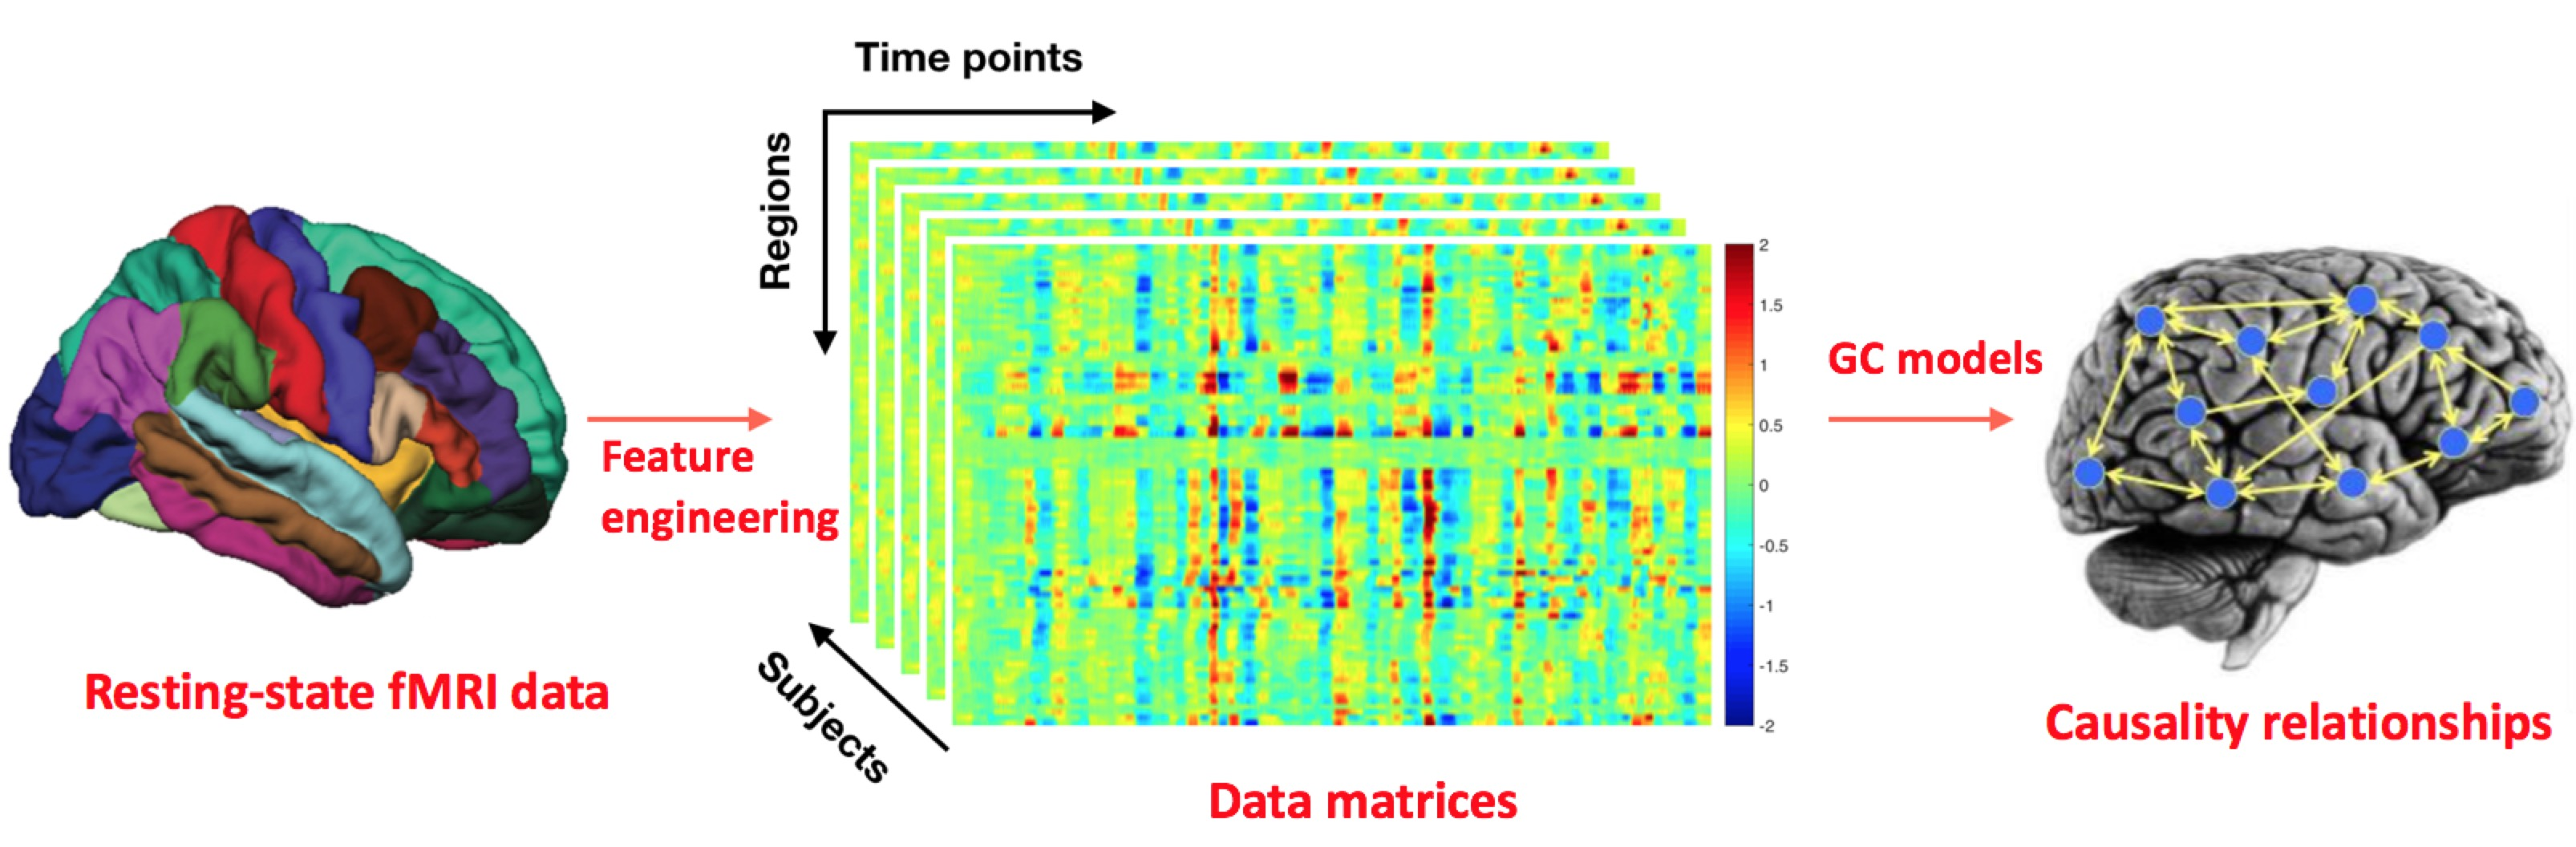
\includegraphics[scale=0.08]{images/task_graph.jpg}
    \vspace{-5mm}
    \caption{Project pipeline: from brain regions to causality networks\label{fig:task_graph}.}
    \vspace{-7mm}
\end{figure}



\section{Spatio-temporal Causal Modeling}
\label{sec:Spatio-temporal}
Modeling the spatio-temporal causality has been widely done using Granger causality. In this section we model the causality between brain regions based on the notion of GC. 

Let's consider ${N}$ nodes, which correspond to brain regions, and ${T}$ time samples which correspond to the time measurements of fMRI. For any time  ${t=0,...,T-1}$ and node ${n=0,...,N-1}$, we can denote the fMRI signal at time  ${t}$ and node  ${n}$ as ${x_{n,t}}$. We can further express the fMRI signal in a matrix $\mathbf{X}$ with ${x_{n,t}}$ in row ${n}$ and column ${t}$.

In order to predict the causality of the time-series we define a lag, ${L}$, which indicates the number of previous samples used for the estimation. Thus, given a node ${i}$, we would like to estimate ${x_{i,t}}$ for ${t=L,...,T-1}$ as
\begin{equation}
\sum_{t=L}^{T-1}x_{i,t}	\approx\sum_{l=1}^{L}{\beta_{l}x_{i,t-l}},
\label{eq:time_causality}
\end{equation}
being ${\beta_{l}}$ the coefficients that weight the contribution of the previous time samples. Note that equation (\ref{eq:time_causality}) is only considering the time causality for a given location while we are interested on the time-spatial causality. In order to take into account the impact of other nodes, equation (\ref{eq:time_causality}) can be reformulated as 
\begin{equation}
\sum_{t=L}^{T-1}x_{i,t}	\approx\sum_{n=0}^{N-1}\sum_{l=1}^{L}{{\beta_i}_{n,l}x_{n,t-l}},
\label{eq:time_causality2}
\end{equation}
where the coefficients not only weight the previous samples impact, but also the nodes. These coefficients are a direct measure of the time-spatial causality and its estimation can be performed by a regression problem.

For each node ${i}$, the coefficients that measure the causality from other nodes to node ${i}$ can be obtained through solving the following problem:
\begin{equation}
{\hat{\boldsymbol\beta}_i}=\operatorname*{argmin}_{\beta_i} \sum_{t=L}^{T-1}(x_{i,t} -\sum_{n=0}^{N-1}\sum_{l=1}^{L}{{\beta_i}_{n,l}x_{n,t-l}})^2+\lambda{\sum_{n=0}^{N-1}\sum_{l=1}^{L}{|{\beta_i}_{n,l}|}},
\label{eq:time_causality3}
\end{equation}
with ${\lambda}$ being the regularization term. It is important mentioning that we are using L1-regularization since we are interested in sparseness, since, for each node, very few others are causal. Note that other techniques such as least-squares or ridge regression would not allow us to control the sparsity of our solution. Equation (\ref{eq:time_causality3}) can be reformulated taking into account more than one data matrices, $\mathbf{X}$ as:
\small
\begin{equation}
{\hat{\boldsymbol\beta}_i}=\operatorname*{argmin}_{\beta_i} \sum_{d=0}^{D-1}\sum_{t=L}^{T-1}(x_{i,t}^d -\sum_{n=0}^{N-1}\sum_{l=1}^{L}{{\beta_i}_{n,l}x_{n,t-l}^d})^2+\lambda{\sum_{n=0}^{N-1}\sum_{l=1}^{L}{|{\beta_i}_{n,l}|}},{}
\label{eq:time_causality4}
\end{equation}
\normalsize
where ${D}$ is the total amount of data matrices and ${x_{n,t}^d}$ the signal coming from the data matrix ${d}$. Problem (\ref{eq:time_causality3}) can be further expressed as
\begin{equation}
{\hat{\Tilde{\boldsymbol\beta}}_i}=\operatorname*{argmin}_{\Tilde{\boldsymbol{\beta_i}}} ||\mathbf{y}-\mathbf{\Tilde{X}}\Tilde{\boldsymbol{\beta_i}}||_2^2+\lambda{||\Tilde{\boldsymbol{\beta_i}}||_1},
\label{eq:time_causality5}
\end{equation}
with

$\mathbf{y}\triangleq[x^0_{i,L},x^0_{i,L+1},...x^0_{i,T-1},x^1_{i,L},...,x^1_{i,T-1},...,x^{D-1}_{i,T-1}]^\mathrm{T}$, $\mathbf{y}\in{\mathbb{R}^{(T-L)D\mathrm{x}1}}$, and $\mathbf{\Tilde{X}}\triangleq[\mathbf{\hat{X}_0},\mathbf{\hat{X}_1},...,\mathbf{\hat{X}_{N-1}}]$,  
\\
\noindent
$\mathbf{\Tilde{X}}\in{\mathbb{R}^{(T-L)D\mathrm{x}LN}}$, where  $\mathbf{\hat{X}_{j}}$ is a matrix defined as

\begin{equation}
\mathbf{\hat{X}_{j}}=\begin{bmatrix}
    x_{j,L-1}^0       & x_{j,L-2}^0 & x_{j,L-3}^0 & \dots & x_{j,L-L}^0 \\
    x_{j,L+1-1}^0       & x_{j,L+1-2}^0 & x_{j,L+1-3}^0 & \dots & x_{j,L+1-L}^0 \\
    \vdots & \vdots & \vdots & \ddots & \vdots \\
    x_{j,T-1-1}^0      & x_{j,T-1-2}^0 & x_{j,T-1-3}^0 & \dots & x_{j,T-1-L}^0 \\
    x_{j,L+1-1}^1       & x_{j,L+1-2}^1 & x_{j,L+1-3}^1 & \dots & x_{j,L+1-L}^1 \\
    \vdots & \vdots & \vdots & \ddots & \vdots \\
   x_{j,T-1-1}^{D-1}      & x_{j,T-1-2}^{D-1} & x_{j,T-1-3}^{D-1} & \dots & x_{j,T-1-L}^{D-1} \\
\end{bmatrix},
\label{eq:time_causality6}
\end{equation}
and $\Tilde{\boldsymbol\beta_i}\triangleq[{\beta_i}_{0,1},...,{\beta_i}_{0,L},{\beta_i}_{1,1},...,{\beta_i}_{1,L},...,{\beta_i}_{N-1,L}]^\mathrm{T}\in{\mathbb{R}^{LN\mathrm{x}1}}$. 

Note that the vector $\Tilde{\boldsymbol\beta}_i$ can be reshaped into a matrix ${\mathbf{B}_i\in{\mathbb{R}^{L\mathrm{x}N}}}$, that contains the causality coefficients from other nodes to node $i$ for ${l=1,...,L}$. 
It is important mentioning that we are not interested in the coefficients $\forall{l}$, instead we want to obtain the relation between nodes. Thus, the causality weight from node ${j}$ to ${i}$ we can be computed for instance by $a_{j,i}=\frac{1}{L}\sum_{l=1}^{L}{{\beta_i}_{j,l}}$ or $a_{j,i}=\operatorname*{max}_{l}{{\beta_i}_{j,l}}$, giving rise to the vector $\mathbf{a_{i}}\triangleq[a_{0,i},...,a_{j,i},...,a_{N-1,i}]^\mathrm{T}$. From performing the estimation of the coefficients for all the nodes, we can easily obtain and adjacency matrix, $\mathbf{A}=[\mathbf{a_{0}},\mathbf{a_{1}},...,\mathbf{a_{N-1}}] \in{\mathbb{R}^{N\mathrm{x}N}}$, which is our ultimate goal.

Moreover, we are neither interested in the self-causality. Thus, problem  (\ref{eq:time_causality6}) for node ${i}$, can be further reduced by compacting the matrices to $\mathbf{\Tilde{X}}\triangleq[\mathbf{\hat{X}_0},...,\mathbf{\hat{X}_{i-1}},\mathbf{\hat{X}_{i+1}},...,\mathbf{\hat{X}_{N-1}}]\in{\mathbb{R}^{(T-L)D\mathrm{x}L(N-1)}}$ and $\Tilde{\boldsymbol\beta_i}\triangleq[{\beta_i}_{0,1},...,{\beta_i}_{0,L},...,{\beta_i}_{i-1,L},{\beta_i}_{i+1,1},...,{\beta_i}_{N-1,L}]^\mathrm{T}\in{\mathbb{R}^{L(N-1)\mathrm{x}1}}$, reducing the overall computation cost and giving rise to a adjacency matrix whose diagonal elements are 0.
 
\section{DATA}
\label{sec:data}

\subsection{Brain data}\label{subsec:braindata}

The data used for this project was obtained from 12 different
subjects. It contains the fMRI signal taken in 12462 voxels and 440 timepoints. Note that the signals are deconvoloved. Since our goal is to obtain the causality between brain regions, the data was parcelled to 90 regional timecourses using the Anatomical Automatic Labeling (AAL) ATLAS \cite{TZOURIOMAZOYER2002273}. Additionally, the lab also provided us 13 innovation-driven co-activation patterns (iCAPs) in the brain from resting-state fMRI. fMRI signals can be decomposed in iCAPS, which reveal spatially and temporally overlapping large-scale networks \cite{icap}. The iCAPs considered are the same than the ones used in \cite{bolton2018interactions}, that correspond to Figure \ref{fig:icapsPaper}.
\begin{figure}
    \centering
    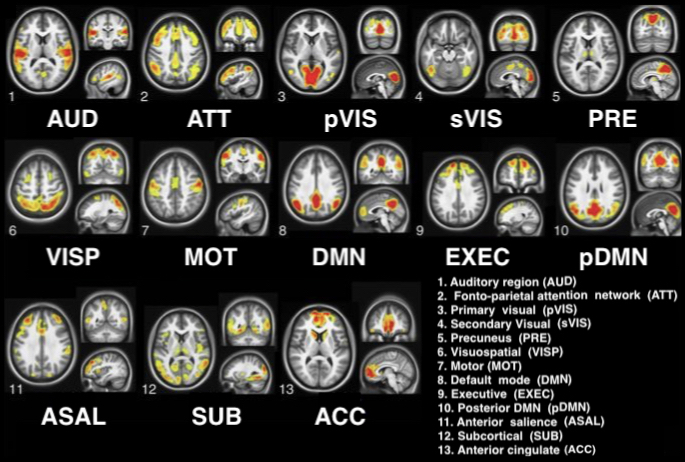
\includegraphics[width=\columnwidth]{images/icaps.jpeg}
    \vspace{-3mm}
    \caption{iCAPs considered. Adapted from \cite{icap}.}
    \label{fig:icapsPaper}
    \vspace{-5mm}
\end{figure}


It is important mentioning that the interpretation of the results when using these databases was complex. In order to proof and optimize our results, we generated synthetic data as it is going to be explained in \ref{var}.

\subsection{VAR model}
\label{var}
In order to make sure our model is working correctly and to allow the possibility of systematic tests we have created our own synthetic data using a VAR model. In each iteration the next row of the matrix is computed using the $L$ rows before that account for the lag. The first $L$ rows are just white Gaussian noise. Let $\mathbf{x_{s,t}}$ denote the row of the matrix of patient $S$ at time $t$. A diagonal of zeros was also imposed to prevent same node causality. We use the following generative model:
\begin{equation}
{\mathbf{x_{s,t}}}=\sum_{l=1}^{L}\mathbf{A_{s,l},\mathbf{x_{s,t-l}}} + \boldsymbol\eta
\label{eq:VAR_model}
\end{equation}

The matrices $\mathbf{A_{s,l}}$ are generated using an adjacency matrix, concerning the relationships between all the nodes, where $A[i,j] = 1$ if there is causality between those nodes in a way that $x_i$ causes $x_j$, and $A[i,j] = 0$ if the nodes are independent. The values for the adjacency matrix are chosen randomly regarding a binomial distribution, where the probability of equaling 0 is 0.8. 

After obtaining the adjacency matrix, we then multiply it by a $\textbf{C}$ matrix, that is created by sampling from a uniform distribution between -0.8 and 0.8. This is done in order to give a random coefficient weight to the nodes that do participate in the causality. 

\subsection{Training the model}
Now that we have both the model and the VAR synthetic data we can begin to test different parameters in order to see which one suits us the best. When using synthetic data the number of nodes is not as high as when using real human data due to the fact that the artificial data being more noisy and random. Therefore, the test that showed were performed using 4 and 6 nodes with a lag of 4. The values demonstrate the mean and standard deviation of 40 test performed for each lambda.


The way the model chooses which nodes have causality is by computing the max value of the different coefficients matrices. After obtaining this final matrix, we change every value that is positively different from 0 to 1, indicating the causality between nodes. The accuracy was calculated, comparing this matrix to the original created adjacency matrix.

\begin{figure}[tbp]
  \centering
  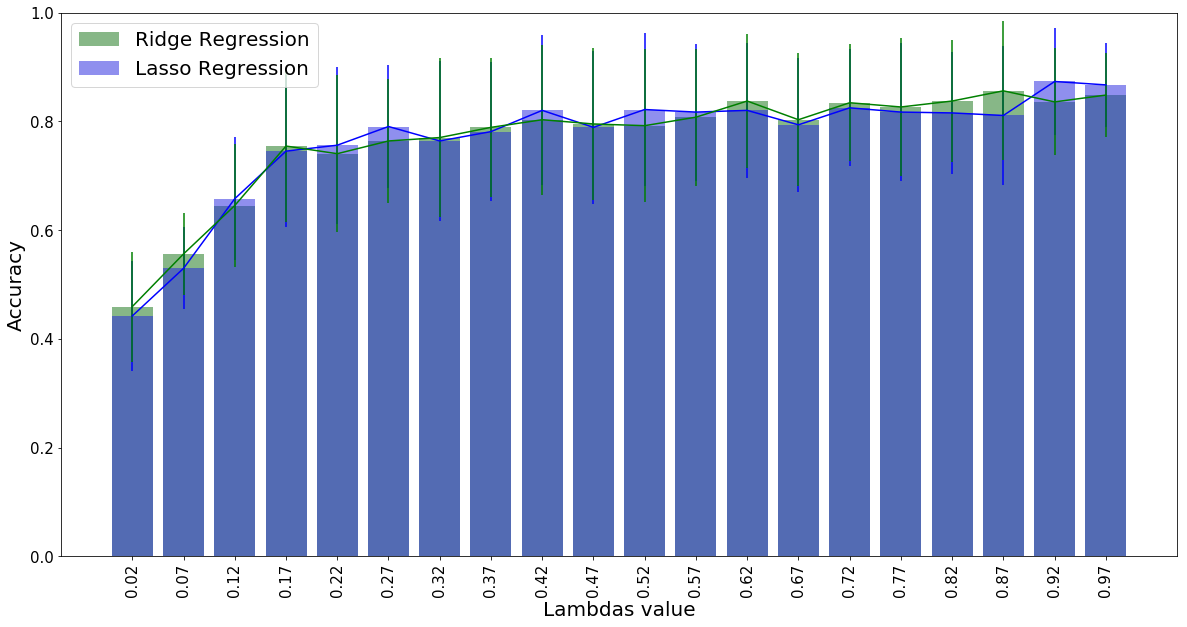
\includegraphics[width=\columnwidth]{images/comaprisonN4_L4.png}
  \vspace{-5mm}
  \caption{Test different lambdas with 4 nodes and a lag of 4.}
  \vspace{-5mm}
  \label{fig:fig:N4L4}
\end{figure}

\begin{figure}[tbp]
  \centering
  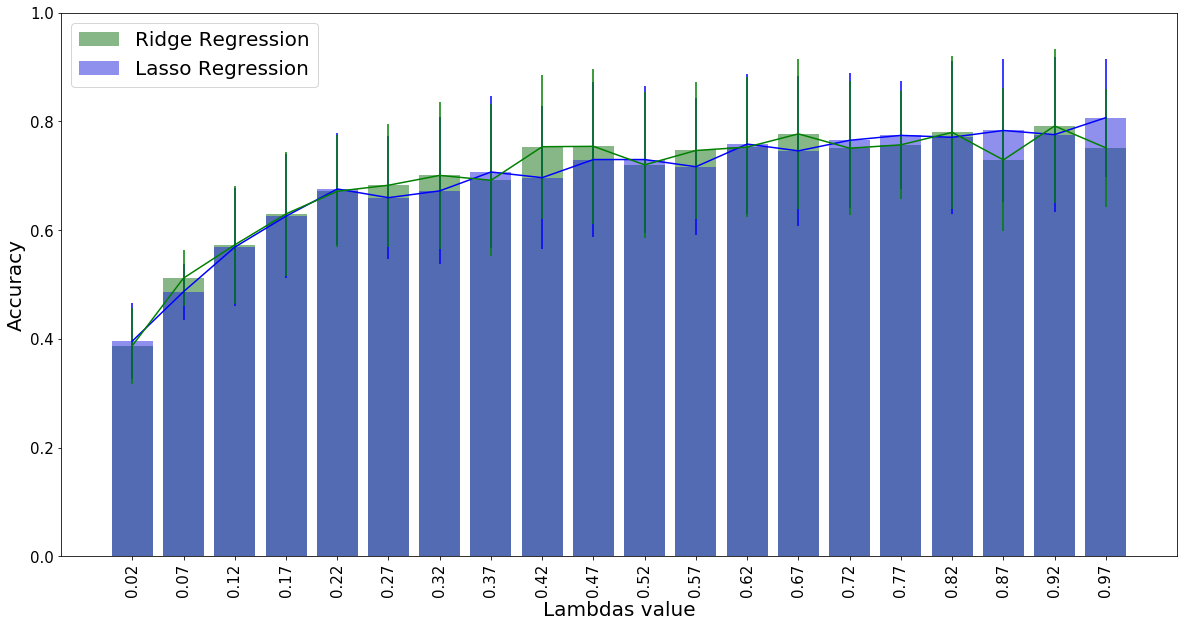
\includegraphics[width=\columnwidth]{images/comaprisonN6_L4.png}
  \vspace{-5mm}
  \caption{Test different lambdas with 6 nodes and a lag of 4.}
  \vspace{-5mm}
  \label{fig:fig:N4L4}
\end{figure}

All of the lambdas and lags tested are not here depicted as we performed a grid search on these parameters. Nevertheless, these images show that we do get good results using lasso and ridge regression, obtaining accuracies of 0.87 and 0.85 for lasso regression using 4 and 6 nodes respectively. Ridge regression does not behave much worse, getting 0.84 and 0.79 using 4 and 6 nodes respectively. You can see that only changing 2 nodes already makes a difference in the accuracy, however our main goal of making sure our model works was achieved with satisfying results. 


The choice between lasso and ridge regression and the different lags does not focus solemnly in this results but also from a biological perspective. Regarding the method it makes more sense to use lasso as it imposes sparsity and it is a prior that makes sense in our case as we know that few nodes are causal. After trying different lags for the real data, the lag of 1 was chosen due to the nature of the data that we are working with, which was sampled every 1 second, being slow compared to neuronal activity and we do not desire to go back in time greatly.


\section{Results}
\label{sec:results}

The coefficients matrix obtained for $L=1$ is shown in Figure \ref{fig:coef}. Combining the coefficients results and by taking into account the iCAPs, we computed for each node in a certain iCAP the number of nodes causing it from another iCAP. As a result, a matrix that relates the 13 different iCAPs by quantifying the causality between them  was obtained as shown in Figure \ref{fig:icaps}.


\begin{figure}%
    \centering
    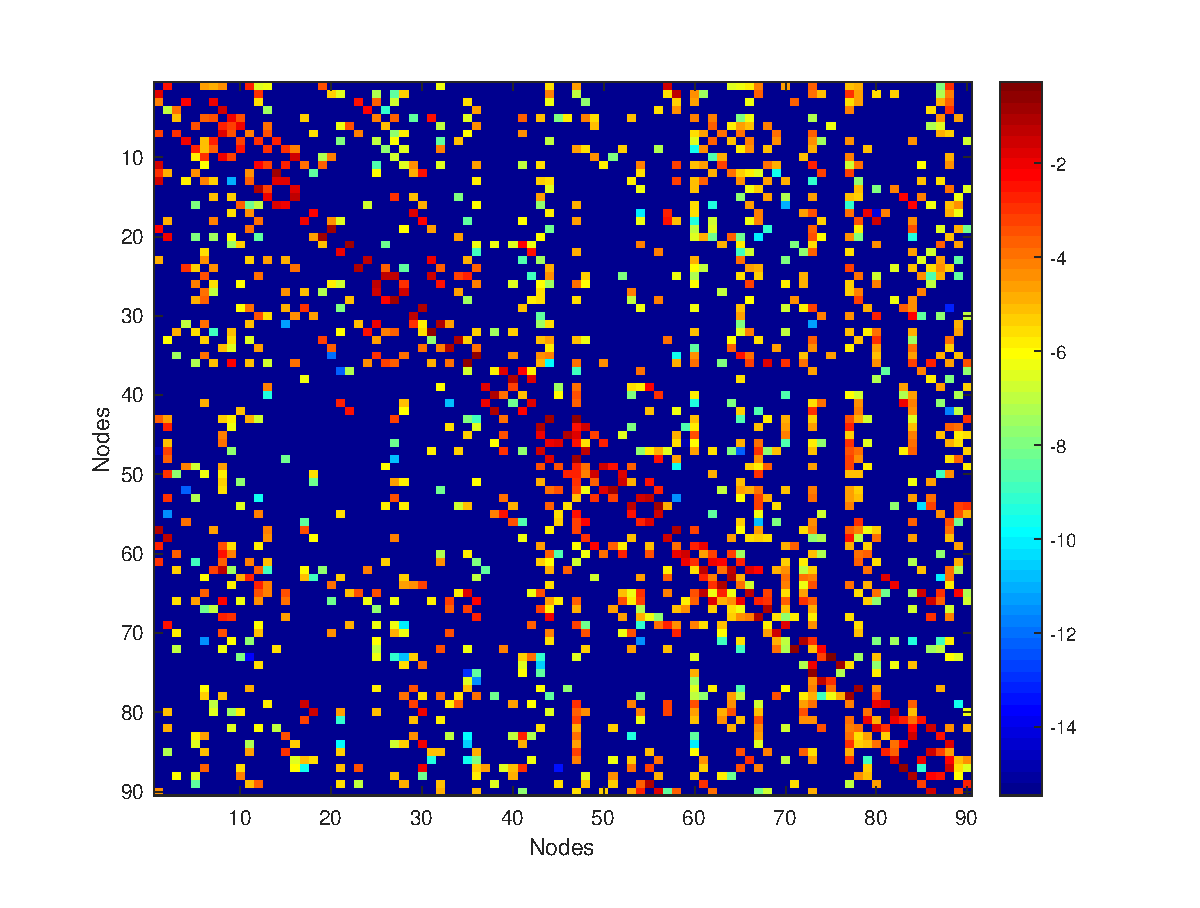
\includegraphics[scale=0.5]{images/coeff.eps}
    \vspace{-5mm}
   % \subfloat[$L=1$]{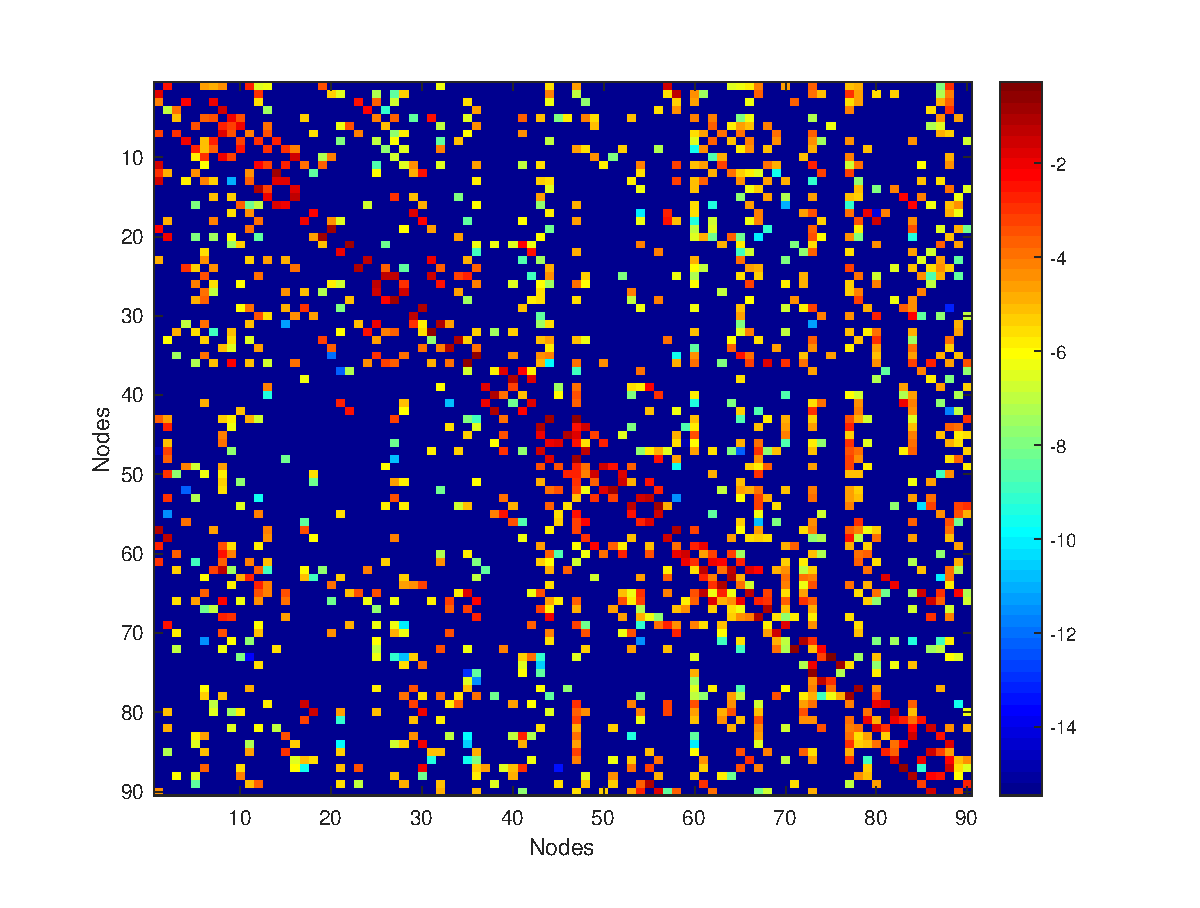
\includegraphics[scale=0.5]{images/coeff.eps}}%
   % \qquad
   % \subfloat[$L=3$]{{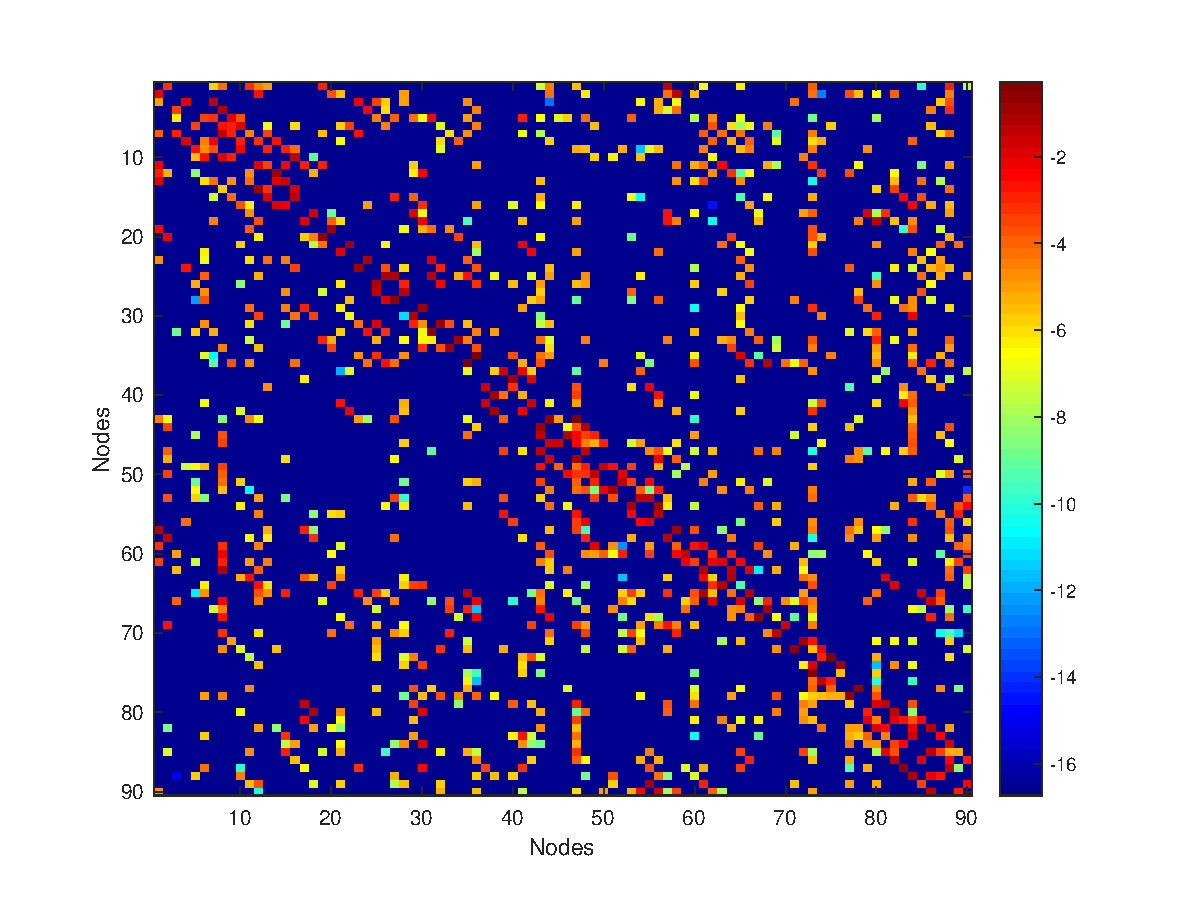
\includegraphics[scale=0.5]{images/coeff_lag3.eps} }}%
    \caption{Coefficients matrix with $L=1$.}%
    \vspace{-7mm}
    \label{fig:coef}%
\end{figure}

\begin{figure}%
    \centering
    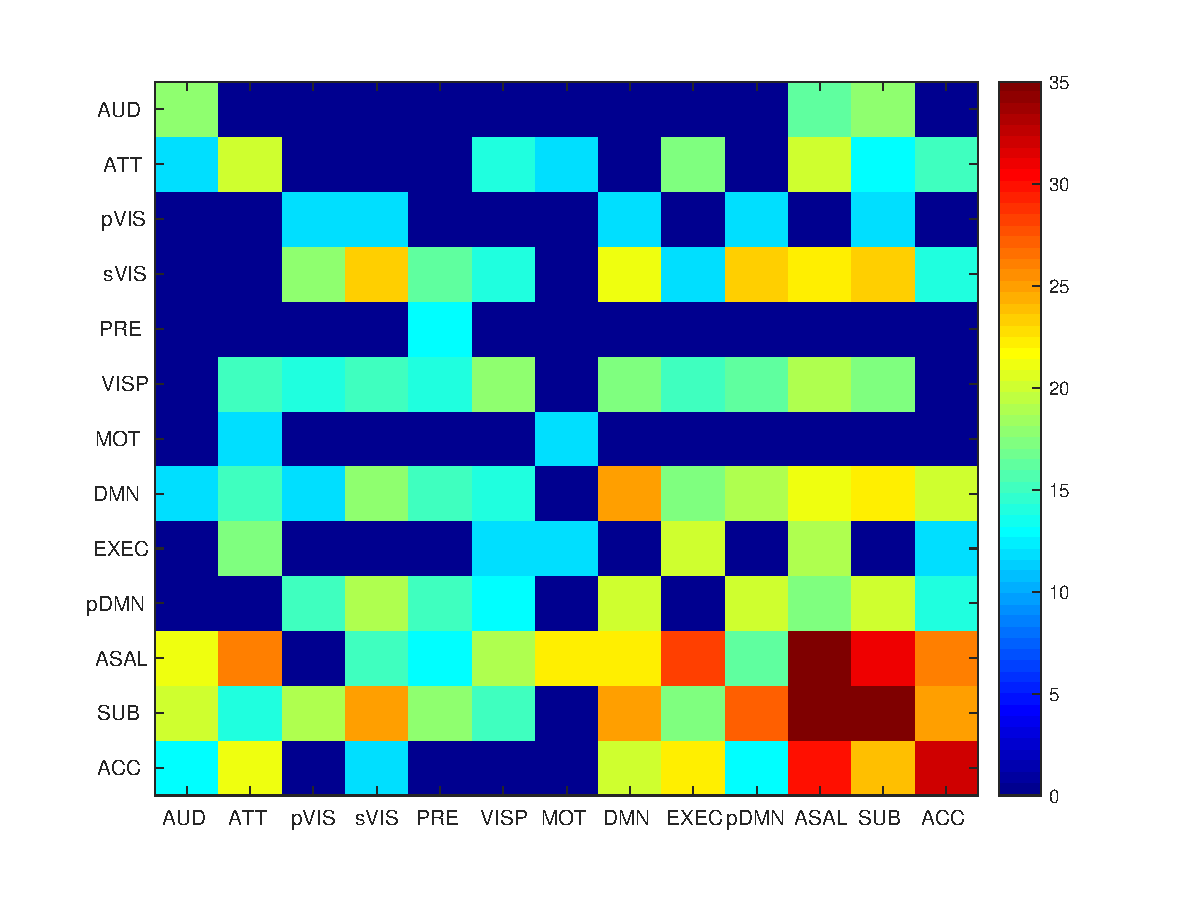
\includegraphics[scale=0.5]{images/icap3.eps}%
   % \hspace{-1cm}
    %\subfloat[$L=3$]{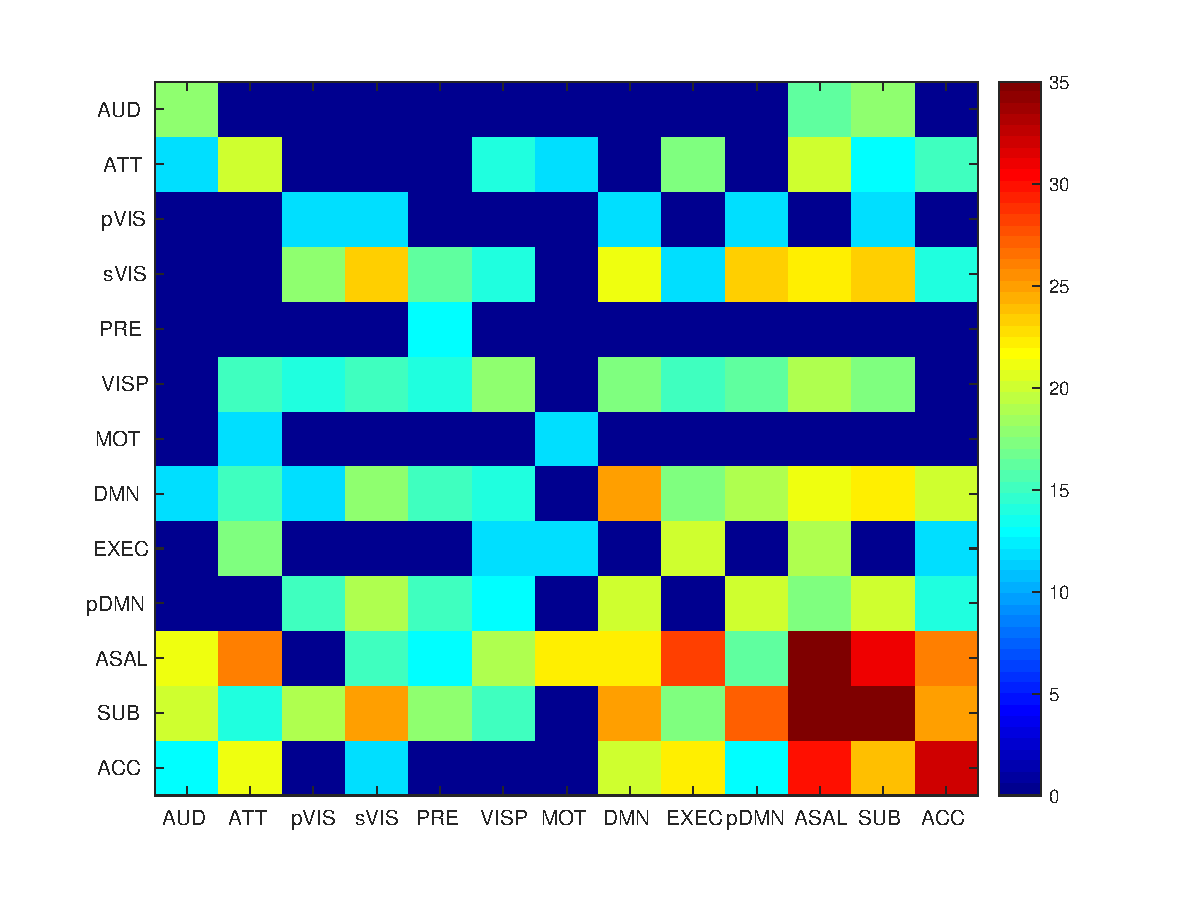
\includegraphics[scale=0.245]{images/icap3.eps} }%
    \vspace{-3mm}
    \caption{Estimated causality matrix for the iCAPs in Figure \ref{fig:icapsPaper}.}%
    \label{fig:icaps}
    \vspace{-3mm}
\end{figure}

 As explained in Section \ref{subsec:braindata}, we are not only interested in causality between nodes, but also between iCAPs. Figure \ref{fig:brain1} shows the nodes that correspond to the primary visual iCAP and the nodes that are known to cause it. Figure  \ref{fig:brain2} represents the estimated causality obtained by combining the obtained coefficients matrix shown in Figure \ref{fig:coef} with the iCAPs nodes in Figure \ref{fig:brain1}.
\begin{figure}%
    \centering
    \subfloat[Nodes\label{fig:brain1}]{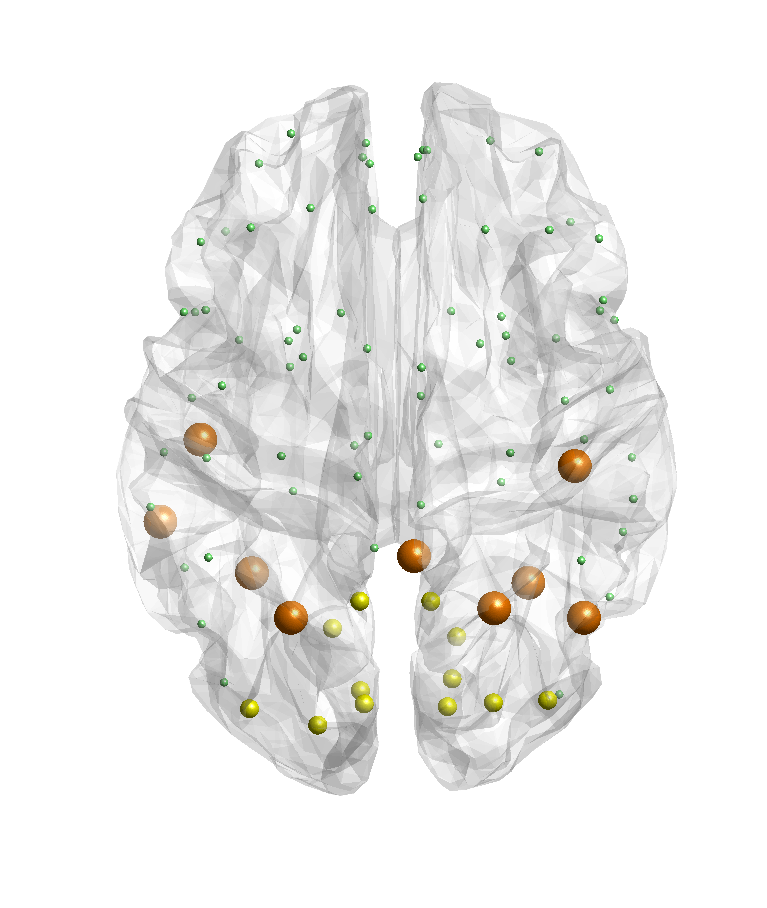
\includegraphics[scale=0.35]{images/visualICAP.eps}}%
    \hspace{0cm}
    \subfloat[Estimated causality\label{fig:brain2}]{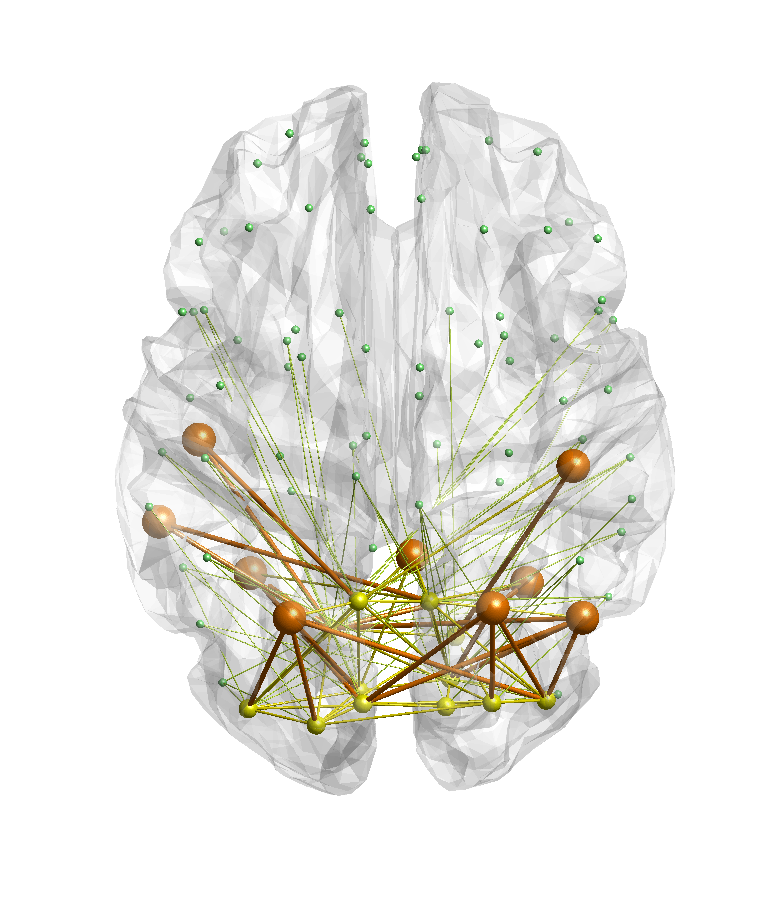
\includegraphics[scale=0.35]{images/estimatedConnections.eps}}%
    \vspace{-2mm}
    \caption{a) iCAPs nodes for primary visual in yellow and nodes that are known to cause it it orange. b) Estimated causality with our approach using lag 1.}%
    \vspace{-8mm}
    \label{fig:brain}%
\end{figure}

For visualization purposes, we have applied a threshold to the matrix in Figure  \ref{fig:icaps} and represented the causality relations in Figure \ref{fig:causal}. Note that we are obtaining similar results than in \cite{bolton2018interactions}, proving the high performance of our approach.

\begin{figure}%
    \centering
    \vspace{-3mm}
    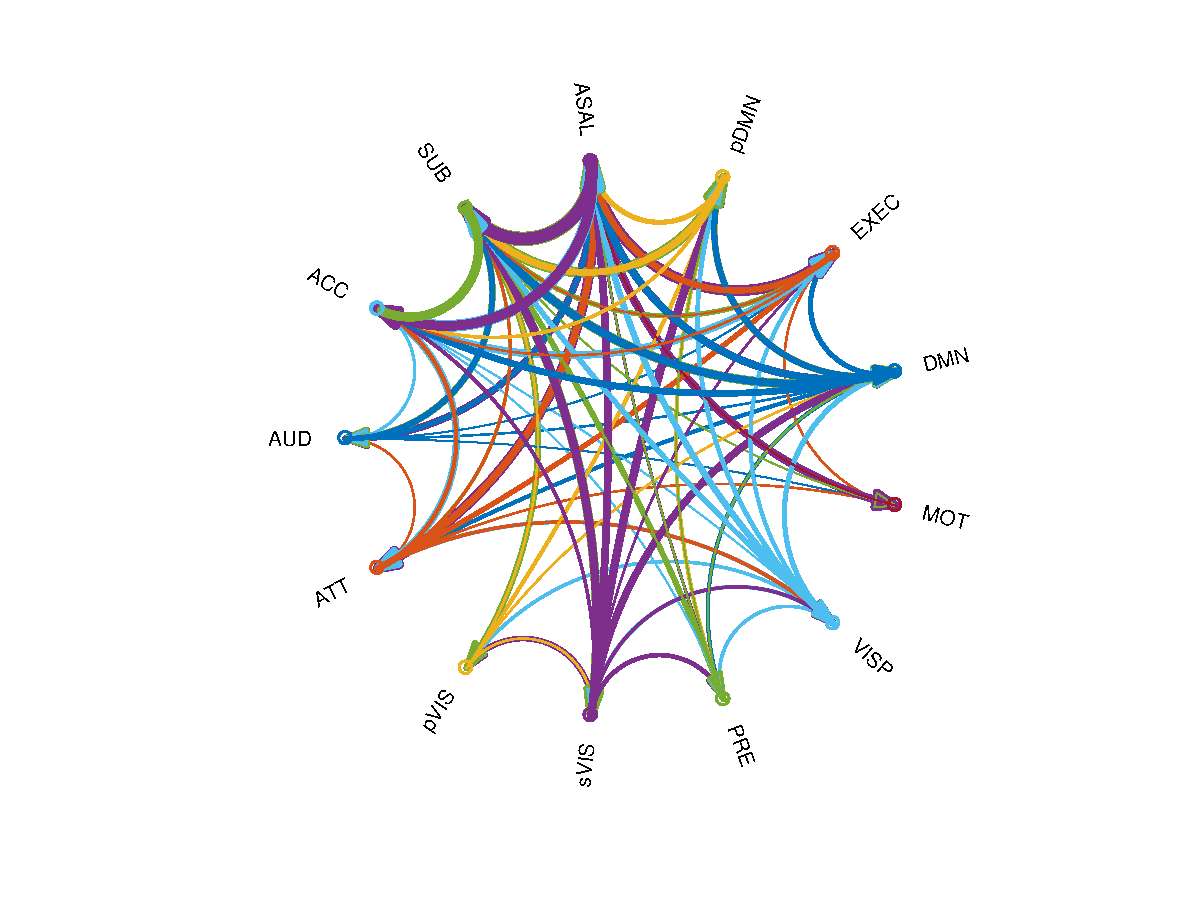
\includegraphics[scale=0.5]{images/th10.eps}%
    \vspace{-10mm}
    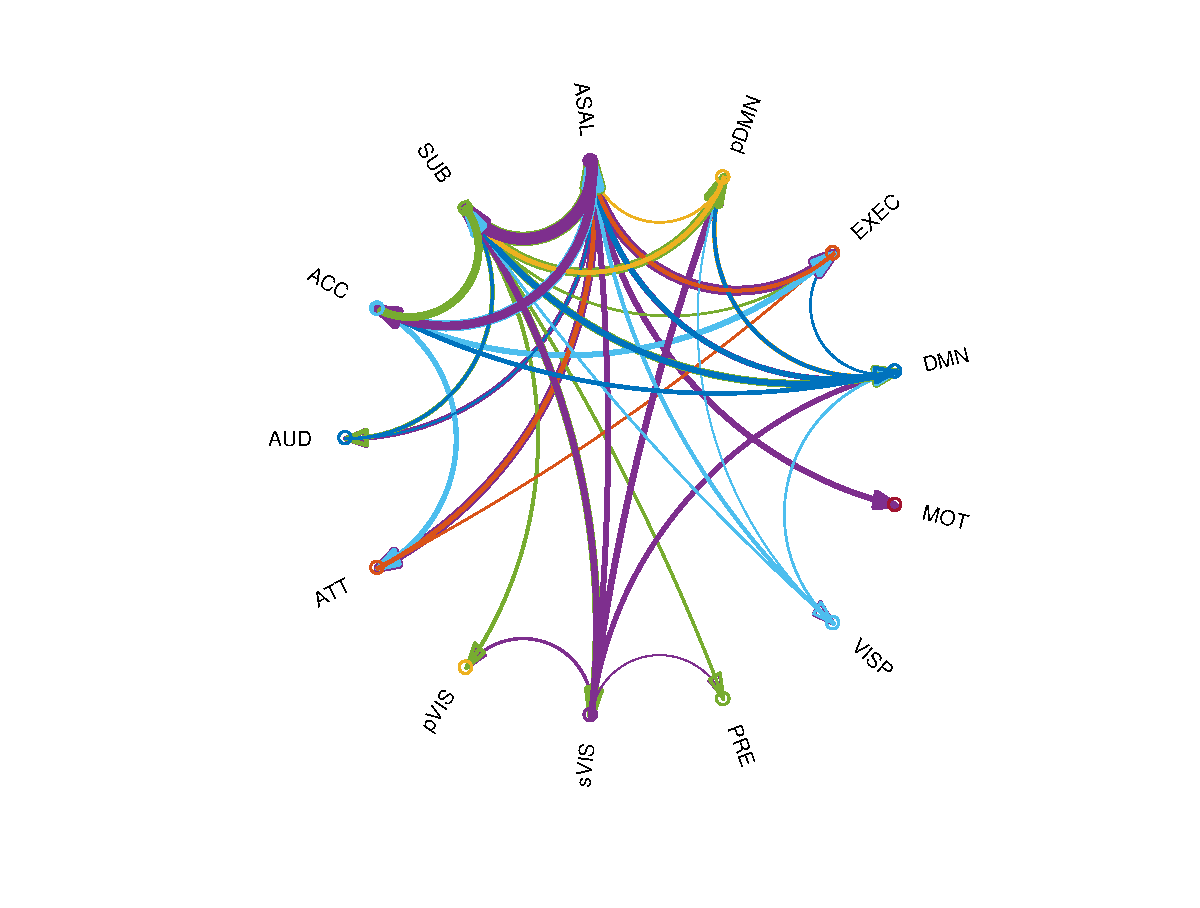
\includegraphics[scale=0.5]{images/th15.eps}
    \vspace{-10mm}
    \caption{Estimated causality between iCAPs by applying two thresholds, 10 and 15, respectively, to the results in Figure \ref{fig:icaps}.}%
    \label{fig:causal}%
\end{figure}

\section{Summary}
\label{sec:summary}
In this paper, we have tackled the estimation of causality between brain regions from resting-state fMRI by applying the concept of Granger causality and formulating a regression problem. First, synthetic data generated with VAR modeling was used to test and optimize our approach. Then, the brain connectivity between 90 regions of the brain was estimated by using deconvolved fMRI signals. Apart from obtaining the causality between these regions, the results were extended to causality between innovation-driven co-activation  patterns, being an innovative approach to studying causality in the brain. As further improvement, we have started including neighborhood information to account also for the spatial dimension.

\bibliographystyle{IEEEtran}
\bibliography{refs} 
\end{document}